\documentclass[12pt]{report}

\usepackage[a4paper, total={6in, 9in}]{geometry}
\usepackage{tikz}
\usepackage{array}
\usepackage{amsthm}
\usepackage{courier}
\usepackage{titlesec}
\usepackage{multibib}
\usepackage{hyperref}
\usepackage{multirow}
\usepackage{arydshln}
\usepackage{enumerate}
\usepackage{hyperref}
\usepackage[dvipsnames]{xcolor}
\graphicspath{ {./images/} }

\hypersetup{colorlinks=true, citecolor=black, linkcolor=black, urlcolor=blue}
\titleformat{\chapter}[display] {\normalfont\Huge\bfseries}{\chaptertitlename\ \thechapter}{0pt}{\Huge}
\titlespacing{\chapter}{0cm}{0cm}{1cm}
\counterwithout{figure}{chapter}
\counterwithout{table}{chapter}
\theoremstyle{definition}
\newtheorem*{example}{Example}
\theoremstyle{definition}
\newtheorem*{algo}{Algorithm}
\theoremstyle{definition}
\newtheorem*{version}{Version}
\providecommand{\keywords}[1]
{\small	\textbf{\textit{Keywords---}} #1}



\begin{document}



\begin{titlepage}
    \newcommand{\HRule}{\rule{\linewidth}{0.5mm}} %Horizontal line break%
    \center
    \textsc{\LARGE Université Toulouse III Paul Sabatier}\\[2.5cm]
    \textsc{\Large Master Thesis Report}\\[0.5cm]
    \textsc{\large Computer Science for Aerospace}\\[2.5cm]

    \HRule\\[0.5cm]
    {\huge \bf Multivariate Decision Tree Classification}\\[0.5cm]
    \HRule\\[1.5cm]

    \begin{minipage}{0.4\textwidth}
		\begin{flushleft}
			\large
			\textit{Author}\\
			Dany Morales
		\end{flushleft}
	\end{minipage}
    \begin{minipage}{0.4\textwidth}
		\begin{flushright}
			\large
			\textit{Supervisors}\\
			Martin Cooper\\
            Emmanuel Hebrard
		\end{flushright}
	\end{minipage}

    \vfill
    \large August 2024

    
\includegraphics[width=0.5\textwidth]{logo.png}
\end{titlepage}



\begin{abstract}
\paragraph{} This report outlines the work accomplished during the second year of a master's thesis in Computer Science for Aerospace, under the supervision of Martin Cooper at the \textit{Institut de Recherche en Informatique de Toulouse (IRIT)} and Emmanuel Hebrard at the \textit{Laboratoire d'Analyse et d'Architecture des Systèmes in Toulouse (LAAS)}. Building upon our previous summer 2023 research project, which involved implementing a heuristic algorithm for multivariate decision tree (MDT) classification, this thesis focuses on the Blossom algorithm, an optimal decision tree (DT) classification method developed by Emmanuel Hebrard. The primary objective is to extend the Blossom algorithm to support MDT's. Using the resulting trees, we explore the notion of abductive explanation (AXp) which reduces the needed number of features to explain a decision of the classifier. The results are analyzed and compared with traditional DT's, demonstrating that MDT's provide equal or greater information while requiring less memory space.\\\\
\keywords{Multivariate Decision Trees, Blossom Algorithm, Abductive Explanation, Feature, Dataset, Classifier}
\end{abstract}



\tableofcontents



\chapter*{Introduction}
During the 2023 summer we developed a heuristic algorithm for MDT classification. With this master thesis we aim to continue working more deeply on MDT's. The main goal of this master thesis is to find a way for the \texttt{Blossom} algorithm developed by Emmanuel Hebrard to support MDT's. We described a lot of notions about DT and MDT classification and existing implementations in a short state of the art in our midterm report.

While we won't go over these notions again, we will briefly reintroduce MDT's and \texttt{Blossom} at the beginning of this report. Then, for each objective we will consider the possible approaches and what results are to be expected before detailing our implemented methods. We will showcase the effectiveness of our solutions in a comprehensive analysis. Through the use of a Student's t-test, we will establish if there is any statistical significance between the accuracy of DT's and MDT's. In turn, we will be able to compare them and confirm or refute our assumptions. 

Finally,  we will highlight links between our thesis and past lectures and put into perspective the work we have accomplished.



\chapter{Multivariate decision trees}
\section{Overview}
\paragraph{} ``A multivariate decision tree is a decision tree in which the condition tested at a node is a constraint on any number of features \cite{multivariate-explaining}.'' The principles of information gain, entropy and Gini impurity from DT's are still valid but, as we introduce another condition to test, finding the best split for each decision node becomes more costly to compute.

\begin{figure}[ht]
    \centering
    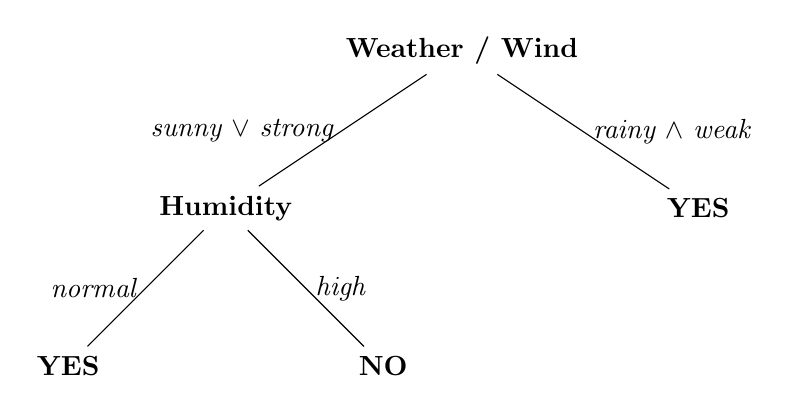
\begin{tikzpicture}
        [
            level 1/.style = {level distance = 2cm, sibling distance = 6cm},
            level 2/.style = {sibling distance = 4cm}
        ]
        
        \node {\bf Weather / Wind}
            child {node {\bf Humidity}
            child {node {\bf YES}
            edge from parent node [left] {\it normal}}
            child {node {\bf NO}
            edge from parent node [right] {\it high}}
            edge from parent node [left] {\it sunny $\lor$ strong}} 
            child {node {\bf YES}
            edge from parent node [right] {\it rainy $\land$ weak}};
    \end{tikzpicture}
    \caption{``\textit{Play outside}'' multivariate decision tree}
    \label{fig:multitree}
\end{figure}

This is a possible MDT that classifies the dataset in table \ref{fig:dataweather}.

\begin{table}[ht]
    \centering
    \begin{tabular}{||c c c c||} 
    \hline
    Weather & Humidity & Wind & Play\\[0.5ex]
    \hline\hline
    Sunny & High & Strong & NO\\ 
    Sunny & Normal & Strong & YES\\
    Rainy & High & Strong & NO\\
    Rainy & High & Weak & YES\\ 
    \hline
    \end{tabular}
    \caption{``\textit{Play outside}'' dataset}
    \label{fig:dataweather}
\end{table}

\paragraph{} The root node test condition is on both the weather and wind features. The left child contains the subset satisfying the condition $weather=sunny \lor wind=strong$ and the right child contains the subset satisfying the negation i.e. $weather=rainy \land wind=weak$. It is important to note that the number of features a condition is testing does not have to be the same at every node.


\section{Blossom algorithm}

\begin{algo}[\texttt{Blossom\cite{blossom}}]
    We take advantage of two properties of decision trees. 
    \begin{enumerate}[(i)]
        \item The set at any decision node is the union of the sets of its children (i.e. the subset of the dataset that satisfies the conditions leading to this node).
        \item The classification result is not changed by the order in which the features are encountered.
    \end{enumerate}
    
    Once the dataset has been split, both sibling subtrees can be optimized independently because of (i). We can take advantage of (ii) when two datasets share the same features by storing results already computed (caching). This approach incentivizes optimizing a subtree before moving to the others.\\

    Similarly to \texttt{MurTree\cite{murtree}}, the \texttt{Blossom} algorithm uses binary datasets and dynamic programming to find optimal decision trees. A significant difference is that before optimizing branches, \texttt{Blossom} always expands branches that did not reach the maximum depth called non-terminal branches or ``blossoms''. This is also an anytime algorithm; it can return a decision tree when interrupted before it ends, as it keeps running, better solutions will be found. \texttt{Blossom} performs better than other state of the art algorithms, especially on deeper trees. Another particularity of this algorithm is the feature reduction applied during preprocessing that will be greatly effective when applied to MDT's.
\end {algo}



\chapter{Work accomplished}
\section{Objectives, approaches and expected results}
\paragraph{} The main objective is to adapt \texttt{Blossom} to support MDT's. Since it is an anytime algorithm, even with a very large dataset and many features, we always expect a result as opposed to traditional heuristic algorithms, thus \texttt{Blossom} is particularly adapted. We can then compare MDT's with DT's and draw some conclusions on their advantages and drawbacks.

We expect MDT's to be significantly more compact while being able to retain roughly the same amount of information, in other words \textbf{we think MDT's are more memory efficient than DT's}.

To achieve this, we have two principal approaches:

\begin{enumerate}[(i)]
    \item Algorithmic approach: change the algorithm code itself
    \item Preprocessing approach: modify the input dataset file
\end{enumerate}

Considering \texttt{Blossom} is written in C++ and we have little experience with this language we chose the approach (ii) which should give similar if not exactly the same results and will be faster to develop.

A secondary objective is to be able to find the average length of abductive explanations (AXp's) from the classified trees. An AXp is a minimal subset of features sufficient to explain a decision of the classifier \cite{multivariate-explaining}. Additionally, we also want to be able to find weak AXp's which are non-minimal subsets of features explaining decisions. This is a fairly straightforward process that we will detail in a dedicated section. Since we need the trees to be classified, this is a postprocessing step.

Finally, \texttt{Blossom} only provides a terminal based way of visualizing the output trees so we also made a program to visualize the trees in a more readable format, which will be useful to make sure our results make sense.


\newpage
\section{Preprocessing}
\paragraph{} We wrote a Python script to expand the features of a binary dataset. The script can add new features of value $a \lor b$ for each possible combination of two distinct features $a$ and $b$ present in the initial dataset.

\begin{example}
    For a dataset containing four features $a$, $b$, $c$ and $d$, the script will add the following six new features: $a \lor b$, $a \lor c$, $a \lor d$, $b \lor c$, $b \lor d$, $c \lor d$.
\end{example}

The number of new features added is $k$ $m \choose 2$ where $m$ is the number of features in the initial dataset and $k$ is the number of conjunctive normal forms (CNF's) used. The other supported CNF's are $(\neg x \lor y)$, $(x \lor \neg y)$, $(\neg x \lor \neg y)$, $(x \oplus y)$. The script allows to expand a dataset with any number of CNF's chosen. The expanded dataset is given in output and is directly ready to use with the \texttt{Blossom} algorithm. It is important to note we do not do extra preprocessing to verify if two features have the same values since \texttt{Blossom} already has some preprocessing steps, including feature reduction that would eliminate any unnecessary or redundant features.

\begin{version}[1] A first version of this program would write into the memory the whole dataset, add the new features and then write the result into a file. This approach is very memory-hungry and is very quickly limited when used on bigger datasets which require multiple gigabytes of RAM.
\end{version}

\begin{version}[2] We made a second version that processes the dataset line by line, for each line, we first put it into the memory, then add the new features and then write it to a file. This way, no matter the size of the dataset, the program only uses a few megabytes of RAM at most and has a constant space complexity. The processing speed is however slightly slowed as a consequence of the multiple read/write system calls we make.
\end{version}

\begin{version}[3] Finally, a third version identical to the second but implemented in C++ providing a significantly faster processing speed, useful for bigger datasets. Additionally, both this and the second versions would greatly benefit from parallelism as they only use a single thread of our processor but we considered it unnecessary. Yet, it would become necessary if we dealt with a dataset multiple gigabytes in size.
\end{version}


\newpage
\section{Postprocessing}
\paragraph{} The first postprocessing we have done is another Python script using the \texttt{Graphviz} library to convert the output tree given by \texttt{Blossom} in the string format and make a more readable tree as an image in the PNG format. 

We can see in figure \ref{fig:viz} a MDT classified using the method described previously. For simplicity we write the conditions inside the nodes. In the left children we have the subsets that satisfy the condition written in the parent node and in the right children we have the subsets that satisfy the negation of the condition written in the parent node. $xN$ represents the feature of index (i.e. column) $N$ in the dataset.

\begin{figure}[ht]
    \centering
    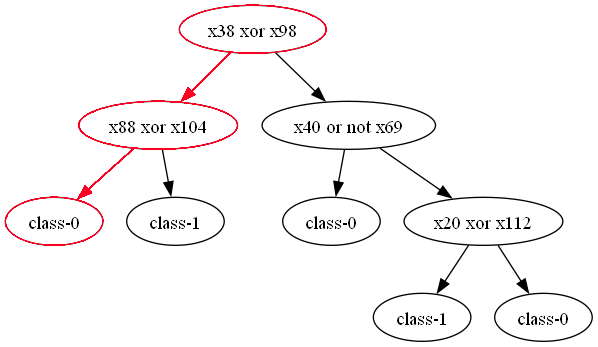
\includegraphics[width=0.75\textwidth]{example.png}
    \caption{Tree visualization}
    \label{fig:viz}
\end{figure}

The next step is to make the link with the research of our supervisor Martin Cooper and find weak AXp's using our MDT's. ``A weak AXp is a set of features that is sufficient to explain the decision, but is not necessarily minimal \cite{multivariate-explaining}.'' What we initially find are a certain type of weak AXp's corresponding to the paths in the trees; we could call them "path explanations". For example, the path explanation corresponding to the red path is the set of four features $\{x38, x98, x88, x104\}$. 

Such path explanations can sometimes be refined by eliminating certain redundant features. The paper demonstrates that explaining a decision can be done in polynomial time by solving a constraint satisfaction problem (CSP) for each leaf-node corresponding to another class. Using our example in figure \ref{fig:viz}, to know whether $\{x38, x88\}$ is a weak AXp of the decision in red, we need to solve CSP's for each leaf-node corresponding to the class 1:
\[ x38=1, x88=1, x38 \oplus x98, \neg (x88 \oplus x104) \]
\[ x38=1, x88=1, \neg (x38 \oplus x98), \neg (x40 \lor \neg x69), x20 \oplus x112 \]

\newpage

\paragraph{} $\{x38, x88\}$ is a weak AXp if and only if each of the corresponding CSP's have no solution. The first CSP has one solution: $\{x38=1, x88=1, x98=0, x104=1\}$, so we can already conclude that $\{x38, x88\}$ is not a weak AXp of the red decision. We can easily solve CSP's in Python using the \texttt{constraint} library which allows us given a decision in a MDT to find weak AXp's and thus be able to explain decisions with fewer features.

\paragraph{} The last postprocessing step is to find the average length of AXp's which we note $Q$ in a tree with $N$ decisions (i.e. leaves). For simplicity, we assume independent uniformly distributed boolean variables, which clearly does not hold if variables are dependent. Let $P_i$ be the proportion of feature vectors which are classified by leaf $i$ and $L_i$ the length of the corresponding AXp, then:

$$Q = \sum_{i=1}^N P_i * L_i$$

\paragraph{} We now need to find the values of $P_i$ for each type of conditions we have: (i) unary, (ii) and, (iii) or, (iv) exclusive or. If $x$ and $y$ are independent boolean variables with a uniform distribution, then:
\begin{enumerate}[(i)]
    \item $P(x=1) = P(y=1) = 1/2$
    \item $P(x=1 \land y=1) = P(x=1) * P(y=1) = 1/4$
    \item $P(x=1 \lor y=1) = 1 - (P(x=0) * P(y=0)) = 3/4$
    \item $P(x=1 \oplus y=1) = P(x=1) * P(y=0) + P(x=0) * P(y=1) = 1/2$
\end{enumerate}

In an explanation, when we have constraints of type: (i) unary, (iii) or, we add 1 to $L_i$. When we have constraints of type: (ii) and, (iv) exclusive or, we add 2 to $L_i$.

\begin{example}
    Using the tree in figure \ref{fig:viz}, if we number the leaves from left to right, the average length of AXp's $Q$ is:\\
    
    $L_1 = L_2 = 4, L_3 = 3, L_4 = L_5 = 6$
    
    $P_1 = P_2 = (1/2) * (1/2) = 1/4$
    
    $P_3 = (1/2) * (3/4) = 3/8$
    
    $P_4 = P_5 = (1/2) * (1/4) * (1/2) = 1/16$

    $Q = 4 * (1/4) + 4 * (1/4) + 3 * (3/8) + 6 * (1/16) + 6 * (1/16) = 3.875$
\end{example}

This computation can easily be added to our program for tree visualization, providing us with more data for further comparison.



\chapter{Analysis of results of experiments}
\section{Discussion}
\paragraph{} In our midterm report, we did some testing to get a rough idea of where MDT's stood compared to DT's and concluded that DT's had a marginally worse accuracy than their multivariate counterparts. This time, our testing is much more rigorous and comprehensive. The goal is to find if we can have more compact trees with the same accuracy and the same average length of AXp's.

We ran \texttt{Blossom} with 12 \textit{normal} datasets and their \textit{expanded} versions for a total of 24 datasets. For each dataset, the classifier had a time limit of 15 minutes which was reached in almost all cases; this approximately amounts to 60 hours of runtime.

We chose to base our testing on depth 7 DT's and depth 5 MDT's because the length of AXP's of DT's of depth $d_1$ is clearly $d_1$ since each node-condition contributes one feature. The expected length of AXp's of MDT's of depth $d_2$ is $d_2 * M$ where $M$ is the average number of features at each node which contribute to an explanation. Assuming that all conditions are binary and that the conditions $x \oplus y$, $x \lor y$, $x \lor \neg y$, $\neg x \lor y$, $\neg x \lor \neg y$ are equally likely:

\[ M = (1/5) * ( 2 + 4 * [ 1 * (3/4) + 2 * (1/4)] ) = (1/5) * 7 = 1.4 \]

Where a XOR condition requires two features, the left branch of an OR condition requires one feature and the right branch (which is the negation) requires two features. Finally, the probability of following the left (respectively right) branch of an OR condition is $3/4$ (respectively $1/4$). Thus, we chose depth 5 DT's which gives us depth $5 * 1.4 = 7$ MDT's so we have round numbers for both depths. 

We first made a Student's t-test to detect if there is a statistical significance between the accuracy of DT's and MDT's. With the result of the t-test, the average length of AXp's and the number of nodes in each tree, we can compare the two types of trees. All the information about the testing hardware, parameters and detailed result tables can be found in the \hyperref[chap:appendix]{appendix}.

\newpage

\section{Student's t-test}
\paragraph{} Our null hypothesis is that there is no difference between DT and MDT accuracy. We are comparing the accuracy achieved with $normal$ datasets and the accuracy achieved with $expanded$ datasets. We made paired two-sample t-tests for both the training accuracy and the testing accuracy. 

The value displayed for the t-test in table \ref{fig:ttest} is the $p$-value i.e. the probability of finding results further from what is expected under the null hypothesis. Essentially, it reflects how unusual or extreme the observed data is if the null hypothesis is true. The smaller the $p$-value, the less likely it is that such extreme results would occur by random chance, which lead to rejecting the null hypothesis. 

We consider the usual threshold of 0.05 for the $p$-value; if we have $p$-value $< 0.05$, then there is a statistical significance in the difference of accuracy between DT's of depth 7 and MDT's of depth 5.

\begin{table}[ht]
    \makebox[\textwidth][c]{
    \begin{tabular}{ccccccc}
    \hline
    \multicolumn{1}{c}{\multirow{2}{*}{\bf seed}} & \multicolumn{3}{c}{\bf training acc.} & \multicolumn{3}{c}{\bf testing acc.} \\
    \multicolumn{1}{c}{} & \multicolumn{1}{p{1.8cm}}{\centering \it normal} & \multicolumn{1}{p{1.8cm}}{\centering \it expanded} & \multicolumn{1}{p{1.8cm}}{\centering \it t-test} & \multicolumn{1}{p{1.8cm}}{\centering \it normal} & \multicolumn{1}{p{1.8cm}}{\centering \it expanded} & \multicolumn{1}{p{1.8cm}}{\centering \it t-test}\\
    \hline
    \multicolumn{1}{c}{1}  & \multicolumn{1}{c}{0.9454} & \multicolumn{1}{c}{0.9255} & \multicolumn{1}{c}{\textcolor{        red}{0.0338}} & \multicolumn{1}{c}{0.8146} & \multicolumn{1}{c}{0.8479} & \multicolumn{1}{c}{\textcolor{        red}{0.0197}} \\
    \multicolumn{1}{c}{2}  & \multicolumn{1}{c}{0.9403} & \multicolumn{1}{c}{0.9248} & \multicolumn{1}{c}{\textcolor{ForestGreen}{0.0976}} & \multicolumn{1}{c}{0.7991} & \multicolumn{1}{c}{0.8110} & \multicolumn{1}{c}{\textcolor{ForestGreen}{0.4133}} \\
    \multicolumn{1}{c}{3}  & \multicolumn{1}{c}{0.9432} & \multicolumn{1}{c}{0.9214} & \multicolumn{1}{c}{\textcolor{        red}{0.0122}} & \multicolumn{1}{c}{0.8083} & \multicolumn{1}{c}{0.8270} & \multicolumn{1}{c}{\textcolor{ForestGreen}{0.1314}} \\
    \multicolumn{1}{c}{4}  & \multicolumn{1}{c}{0.9453} & \multicolumn{1}{c}{0.9252} & \multicolumn{1}{c}{\textcolor{        red}{0.0165}} & \multicolumn{1}{c}{0.8187} & \multicolumn{1}{c}{0.8322} & \multicolumn{1}{c}{\textcolor{ForestGreen}{0.2984}} \\
    \multicolumn{1}{c}{5}  & \multicolumn{1}{c}{0.9453} & \multicolumn{1}{c}{0.9238} & \multicolumn{1}{c}{\textcolor{        red}{0.0067}} & \multicolumn{1}{c}{0.8187} & \multicolumn{1}{c}{0.8267} & \multicolumn{1}{c}{\textcolor{ForestGreen}{0.3464}} \\
    \multicolumn{1}{c}{6}  & \multicolumn{1}{c}{0.9465} & \multicolumn{1}{c}{0.9184} & \multicolumn{1}{c}{\textcolor{        red}{0.0092}} & \multicolumn{1}{c}{0.8021} & \multicolumn{1}{c}{0.8281} & \multicolumn{1}{c}{\textcolor{ForestGreen}{0.1127}} \\
    \multicolumn{1}{c}{7}  & \multicolumn{1}{c}{0.9438} & \multicolumn{1}{c}{0.9218} & \multicolumn{1}{c}{\textcolor{        red}{0.0096}} & \multicolumn{1}{c}{0.8106} & \multicolumn{1}{c}{0.8388} & \multicolumn{1}{c}{\textcolor{        red}{0.0229}} \\
    \multicolumn{1}{c}{8}  & \multicolumn{1}{c}{0.9460} & \multicolumn{1}{c}{0.9235} & \multicolumn{1}{c}{\textcolor{        red}{0.0199}} & \multicolumn{1}{c}{0.8203} & \multicolumn{1}{c}{0.8426} & \multicolumn{1}{c}{\textcolor{ForestGreen}{0.0672}} \\
    \multicolumn{1}{c}{9}  & \multicolumn{1}{c}{0.9472} & \multicolumn{1}{c}{0.9281} & \multicolumn{1}{c}{\textcolor{        red}{0.0236}} & \multicolumn{1}{c}{0.8213} & \multicolumn{1}{c}{0.8310} & \multicolumn{1}{c}{\textcolor{ForestGreen}{0.2115}} \\
    \multicolumn{1}{c}{10} & \multicolumn{1}{c}{0.9467} & \multicolumn{1}{c}{0.9204} & \multicolumn{1}{c}{\textcolor{        red}{0.0093}} & \multicolumn{1}{c}{0.8129} & \multicolumn{1}{c}{0.8250} & \multicolumn{1}{c}{\textcolor{ForestGreen}{0.2412}} \\
    \hline
    \multicolumn{1}{c}{\bf Average} & \multicolumn{1}{c}{\bf 0.9449} & \multicolumn{1}{c}{\bf 0.9232} & \multicolumn{1}{c}{\textcolor{red}{\bf 0.0238}} & \multicolumn{1}{c}{\bf 0.8126} & \multicolumn{1}{c}{\bf 0.8310} & \multicolumn{1}{c}{\textcolor{ForestGreen}{\bf 0.1864}} \\
    \hline
    \end{tabular}}
    \caption{T-test comparing the accuracy of \textit{normal} and \textit{expanded} datasets with \texttt{Blossom} for $seed=[1..10]$}
    \label{fig:ttest}
\end{table}

For the training accuracy, we achieve better accuracy with $normal$ datasets than with their $expanded$ counterparts. In all seeds except the second seed, we reject the null hypothesis and consider the difference in accuracy is statistically significant.

On the contrary, the testing accuracy is higher when using $expanded$ datasets compared to $normal$ datasets and the t-tests confirm that there is no real statistical significance except for two seeds, but even in those cases, it would mean MDT's are more accurate than DT's.

At first, it is strange to have contradicting results between training and testing accuracy. This can be explained by the fact that DT's are overfitting since they perform better in training than testing.

In supervised learning, the testing accuracy is generally considered more crucial so our conclusion is that there is no difference between depth 7 DT and depth 5 MDT accuracy.


\section{Comparison}
\paragraph{} The final step of our testing is comparing trees obtained with both types of datasets. We compare depth 7 DT's classified using $normal$ datasets and depth 5 MDT's classified using $expanded$ datasets. The comparisons are made on:

\begin{enumerate}[(i)]
    \item testing accuracy
    \item average AXp length
    \item total number of node in the tree (i.e. size of the tree)
\end{enumerate} 

\begin{table}[ht]
    \makebox[\textwidth][c]{
    \begin{tabular}{lcccccc}
    \hline
    \multicolumn{1}{l}{\multirow{2}{*}{\bf dataset}} & \multicolumn{2}{c}{\bf testing acc.} & \multicolumn{2}{c}{\bf AXp length avg.} & \multicolumn{2}{c}{\bf node count} \\
    \multicolumn{1}{l}{} & \multicolumn{1}{p{1.8cm}}{\centering \it normal} & \multicolumn{1}{p{1.8cm}}{\centering \it expanded} & \multicolumn{1}{p{1.8cm}}{\centering \it normal} & \multicolumn{1}{p{1.8cm}}{\centering \it expanded} & \multicolumn{1}{p{1.8cm}}{\centering \it normal} & \multicolumn{1}{p{1.8cm}}{\centering \it expanded} \\
    \hline
    \multicolumn{1}{l}{\tt anneal}        & \multicolumn{1}{c}{0.8711} & \multicolumn{1}{c}{0.8650} & \multicolumn{1}{c}{3.71} & \multicolumn{1}{c}{2.40} & \multicolumn{1}{c}{103} & \multicolumn{1}{c}{31} \\
    \multicolumn{1}{l}{\tt breast-cancer} & \multicolumn{1}{c}{0.8978} & \multicolumn{1}{c}{0.9562} & \multicolumn{1}{c}{3.78} & \multicolumn{1}{c}{3.79} & \multicolumn{1}{c}{ 49} & \multicolumn{1}{c}{29} \\
    \multicolumn{1}{l}{\tt car}           & \multicolumn{1}{c}{0.9682} & \multicolumn{1}{c}{0.9768} & \multicolumn{1}{c}{4.90} & \multicolumn{1}{c}{2.59} & \multicolumn{1}{c}{107} & \multicolumn{1}{c}{29} \\
    \multicolumn{1}{l}{\tt diabetes}      & \multicolumn{1}{c}{0.6623} & \multicolumn{1}{c}{0.7597} & \multicolumn{1}{c}{6.64} & \multicolumn{1}{c}{6.42} & \multicolumn{1}{c}{223} & \multicolumn{1}{c}{53} \\
    \multicolumn{1}{l}{\tt forest-fires}  & \multicolumn{1}{c}{0.5192} & \multicolumn{1}{c}{0.5384} & \multicolumn{1}{c}{4.14} & \multicolumn{1}{c}{3.86} & \multicolumn{1}{c}{ 75} & \multicolumn{1}{c}{29} \\
    \multicolumn{1}{l}{\tt hypothyroid}   & \multicolumn{1}{c}{0.9738} & \multicolumn{1}{c}{0.9769} & \multicolumn{1}{c}{4.57} & \multicolumn{1}{c}{5.48} & \multicolumn{1}{c}{109} & \multicolumn{1}{c}{45} \\
    \multicolumn{1}{l}{\tt ionosphere}    & \multicolumn{1}{c}{0.9154} & \multicolumn{1}{c}{0.9436} & \multicolumn{1}{c}{3.48} & \multicolumn{1}{c}{4.70} & \multicolumn{1}{c}{ 41} & \multicolumn{1}{c}{25} \\
    \multicolumn{1}{l}{\tt lymph}         & \multicolumn{1}{c}{0.7741} & \multicolumn{1}{c}{0.9032} & \multicolumn{1}{c}{3.60} & \multicolumn{1}{c}{4.14} & \multicolumn{1}{c}{ 31} & \multicolumn{1}{c}{21} \\
    \multicolumn{1}{l}{\tt messidor-bin}  & \multicolumn{1}{c}{0.6753} & \multicolumn{1}{c}{0.6969} & \multicolumn{1}{c}{5.95} & \multicolumn{1}{c}{6.75} & \multicolumn{1}{c}{179} & \multicolumn{1}{c}{63} \\
    \multicolumn{1}{l}{\tt pendigits}     & \multicolumn{1}{c}{0.9973} & \multicolumn{1}{c}{0.9973} & \multicolumn{1}{c}{3.98} & \multicolumn{1}{c}{5.30} & \multicolumn{1}{c}{ 37} & \multicolumn{1}{c}{29} \\
    \multicolumn{1}{l}{\tt titanic}       & \multicolumn{1}{c}{0.7696} & \multicolumn{1}{c}{0.8089} & \multicolumn{1}{c}{5.35} & \multicolumn{1}{c}{5.42} & \multicolumn{1}{c}{129} & \multicolumn{1}{c}{39} \\
    \multicolumn{1}{l}{\tt yeast}         & \multicolumn{1}{c}{0.7516} & \multicolumn{1}{c}{0.7516} & \multicolumn{1}{c}{5.53} & \multicolumn{1}{c}{6.41} & \multicolumn{1}{c}{175} & \multicolumn{1}{c}{57} \\
    \hline
    \multicolumn{1}{l}{\bf Average}       & \multicolumn{1}{c}{\bf 0.8146} & \multicolumn{1}{c}{\bf 0.8479} & \multicolumn{1}{c}{\bf 4.64} & \multicolumn{1}{c}{\bf 4.77} & \multicolumn{1}{c}{\bf 104.8} & \multicolumn{1}{c}{\bf 37.5} \\
    \hline
    \end{tabular}}
    \caption{Comparison of \texttt{Blossom} between \textit{normal} and \textit{expanded} datasets for \\ $seed=1$}
    \label{fig:comparison}
\end{table}

Even though the testing accuracy seems higher for $expanded$ datasets, we established that there is no statistically significant difference. The average length of AXp's is virtually the same. However, the number of nodes in MDT's is dramatically lower than in DT's, by almost a factor of three. This makes sense since DT's are of depth 7 and MDT's are of depth 5; deeper trees have an increased number of nodes.

We can now confirm our assumptions that given the right depth in parameter, MDT's have equivalent testing accuracy and AXp length than DT's while requiring less nodes. This means that MDT's are more compact but this also means that they can store as much if not more information using less memory space.



\chapter{Appraisal}
\section{Thesis-lecture parallel}
\paragraph{} Throughout our thesis we encountered situations in which content of lectures seen during the master supported our work. We showcased such parallels in table \ref{fig:parallels}.

\begin{table}[ht]
    \centering
    \begin{tabular}{cc}
    \hline
    \multicolumn{1}{p{6cm}}{\centering \bf Topic encountered} & \multicolumn{1}{p{6cm}}{\centering\bf Teaching unit} \\
    \hline
    \multicolumn{1}{p{6cm}}{\centering Binary trees\\Constraint satisfaction problem} & \multicolumn{1}{c}{\multirow{2}{*}{Advanced Algorithmic [M1]}} \\
    \hline
    \multicolumn{1}{c}{\multirow{2}{*}{Decision tree classification}} & \multicolumn{1}{p{6cm}}{\centering Scientific Computing and Machine Learning [M2]} \\
    \hline
    \multicolumn{1}{p{6cm}}{\centering Possibility of improvement (multithreading/parallelism)} & \multicolumn{1}{c}{\multirow{2}{*}{Parallelism [M1]}} \\
    \hline
    \end{tabular}
    \caption{Thesis-lecture parallel}
    \label{fig:parallels}
\end{table}


\section{Broader perspective}
\paragraph{} We showed that MDT's are more accurate in testing as well as more memory efficient than DT's. Although more practical than theoretical, our work is a small contribution to MDT research.

All things considered, our practical oriented approach revealed that \textit{all} DT classification algorithms can be adapted to support MDT's through the alteration of their input datasets.

On a personal level, the work accomplished deepened our technical knowledge of supervised learning for decision trees and data manipulation in Python. Moreover, we trained on a language we never used before by translating our expansion script to C++.



\chapter*{Conclusion}
\paragraph{} In a nutshell, we recalled the basics of MDT's and the functioning of the \texttt{Blossom} classifier developed by Emmanuel Hebrard. Our principal objective was to demonstrate that MDT's are more compact while maintaining the same accuracy and average AXp length as DT's. Two side goals were to allow for better visualization of output trees and making a link with Martin Cooper's research by finding weak AXp's using our MDT's.

We detailed the challenges encountered and how we solved them by developing several versions of our preprocessing script taking $normal$ datasets and adding CNF's of their features creating an $expanded$ dataset. Our 3-step postprocessing permitted us to: clearly picture trees outputted by \texttt{Blossom}, find weak AXp's and finally compute the average AXp length.

In an analysis proving that there is no difference in testing accuracy between MDT's and DT's using a Student's t-test, we were able to compare depth 7 DT's with depth 5 MDT's and conclude that MDT's retained at least the same amount of information while being more memory efficient.

Finally, we reflected on the work accomplished displaying the lectures that assisted us and eventually, we put everything into perspective by understanding how we contributed to multivariate decision tree research and what we achieved on a personal level.

\vspace{9.5cm}

\textit{Thanks to both Martin Cooper and Emmanuel Hebrard for their help and availability throughout the master thesis.}



\nocite{*}
\bibliographystyle{unsrt}
\bibliography{references}



\appendix
\chapter*{Appendix}
\label{chap:appendix}
All our code and the traces of the \texttt{Blossom} algorithm for our tests as well as the code for this report can be found on \href{https://github.com/Selarow/blossom}{GitHub}.


\section*{Experimental results}
\paragraph{} All the accuracy tables can be found below for $seed=[1..10]$. The parameters for each execution are detailed in table \ref{fig:parameters}. \\

\begin{table}[ht]
    \centering
    \begin{tabular}{lcc}
    \hline
    \multicolumn{1}{l}{\bf parameter} & \multicolumn{1}{p{2cm}}{\centering \it normal} & \multicolumn{1}{p{2cm}}{\centering \it expanded} \\
    \hline
    \multicolumn{1}{l}{\tt maxdepth}   & \multicolumn{1}{c}{  7} & \multicolumn{1}{c}{5} \\
    \multicolumn{1}{l}{\tt testsample} & \multicolumn{1}{c}{0.2} & \multicolumn{1}{c}{0.2} \\
    \multicolumn{1}{l}{\tt time}       & \multicolumn{1}{c}{900} & \multicolumn{1}{c}{900} \\
    \hline
    \end{tabular}
    \caption{Parameters used for the execution of \texttt{Blossom}}
    \label{fig:parameters}
\end{table}

\it Benchmarks done using Intel(R) Core(TM) i7-8700K with Windows Subsystem for Linux.
\\\\\\\\\\\\

\begin{table}[ht]
    \centering
    \begin{tabular}{lcccc}
    \hline
    \multicolumn{1}{l}{\multirow{2}{*}{\bf dataset}} & \multicolumn{2}{c}{\bf training acc.} & \multicolumn{2}{c}{\bf testing acc.} \\
    \multicolumn{1}{l}{} & \multicolumn{1}{p{2cm}}{\centering \it normal} & \multicolumn{1}{p{2cm}}{\centering \it expanded} & \multicolumn{1}{p{2cm}}{\centering \it normal} & \multicolumn{1}{p{2cm}}{\centering \it expanded} \\
    \hline
    \multicolumn{1}{l}{\tt anneal}        & \multicolumn{1}{c}{0.9368} & \multicolumn{1}{c}{0.9121} & \multicolumn{1}{c}{0.8711} & \multicolumn{1}{c}{0.8650} \\
    \multicolumn{1}{l}{\tt breast-cancer} & \multicolumn{1}{c}{1.0000} & \multicolumn{1}{c}{1.0000} & \multicolumn{1}{c}{0.8978} & \multicolumn{1}{c}{0.9562} \\
    \multicolumn{1}{l}{\tt car}           & \multicolumn{1}{c}{0.9942} & \multicolumn{1}{c}{0.9913} & \multicolumn{1}{c}{0.9682} & \multicolumn{1}{c}{0.9768} \\
    \multicolumn{1}{l}{\tt diabetes}      & \multicolumn{1}{c}{0.9918} & \multicolumn{1}{c}{0.9006} & \multicolumn{1}{c}{0.6623} & \multicolumn{1}{c}{0.7597} \\
    \multicolumn{1}{l}{\tt forest-fires}  & \multicolumn{1}{c}{0.7675} & \multicolumn{1}{c}{0.7675} & \multicolumn{1}{c}{0.5192} & \multicolumn{1}{c}{0.5384} \\
    \multicolumn{1}{l}{\tt hypothyroid}   & \multicolumn{1}{c}{0.9942} & \multicolumn{1}{c}{0.9922} & \multicolumn{1}{c}{0.9738} & \multicolumn{1}{c}{0.9769} \\
    \multicolumn{1}{l}{\tt ionosphere}    & \multicolumn{1}{c}{1.0000} & \multicolumn{1}{c}{1.0000} & \multicolumn{1}{c}{0.9154} & \multicolumn{1}{c}{0.9436} \\
    \multicolumn{1}{l}{\tt lymph}         & \multicolumn{1}{c}{1.0000} & \multicolumn{1}{c}{1.0000} & \multicolumn{1}{c}{0.7741} & \multicolumn{1}{c}{0.9032} \\
    \multicolumn{1}{l}{\tt messidor-bin}  & \multicolumn{1}{c}{0.8500} & \multicolumn{1}{c}{0.8119} & \multicolumn{1}{c}{0.6753} & \multicolumn{1}{c}{0.6969} \\
    \multicolumn{1}{l}{\tt pendigits}     & \multicolumn{1}{c}{1.0000} & \multicolumn{1}{c}{1.0000} & \multicolumn{1}{c}{0.9973} & \multicolumn{1}{c}{0.9973} \\
    \multicolumn{1}{l}{\tt titanic}       & \multicolumn{1}{c}{0.9337} & \multicolumn{1}{c}{0.8998} & \multicolumn{1}{c}{0.7696} & \multicolumn{1}{c}{0.8089} \\
    \multicolumn{1}{l}{\tt yeast}         & \multicolumn{1}{c}{0.8768} & \multicolumn{1}{c}{0.8305} & \multicolumn{1}{c}{0.7516} & \multicolumn{1}{c}{0.7516} \\
    \hline
    \multicolumn{1}{l}{\bf Average}       & \multicolumn{1}{c}{\bf 0.9454} & \multicolumn{1}{c}{\bf 0.9255} & \multicolumn{1}{c}{\bf 0.8146} & \multicolumn{1}{c}{\bf 0.8479} \\
    \hline
    \end{tabular}
    \caption{Accuracy of \texttt{Blossom} with \textit{normal} and \textit{expanded} datasets for $seed=1$}
    \label{fig:seed1}
\end{table}

\begin{table}[ht]
    \centering
    \begin{tabular}{lcccc}
    \hline
    \multicolumn{1}{l}{\multirow{2}{*}{\bf dataset}} & \multicolumn{2}{c}{\bf training acc.} & \multicolumn{2}{c}{\bf testing acc.} \\
    \multicolumn{1}{l}{} & \multicolumn{1}{p{2cm}}{\centering \it normal} & \multicolumn{1}{p{2cm}}{\centering \it expanded} & \multicolumn{1}{p{2cm}}{\centering \it normal} & \multicolumn{1}{p{2cm}}{\centering \it expanded} \\
    \hline
    \multicolumn{1}{l}{\tt anneal}        & \multicolumn{1}{c}{0.9399} & \multicolumn{1}{c}{0.9198} & \multicolumn{1}{c}{0.8711} & \multicolumn{1}{c}{0.8773} \\
    \multicolumn{1}{l}{\tt breast-cancer} & \multicolumn{1}{c}{1.0000} & \multicolumn{1}{c}{1.0000} & \multicolumn{1}{c}{0.8978} & \multicolumn{1}{c}{0.9124} \\
    \multicolumn{1}{l}{\tt car}           & \multicolumn{1}{c}{0.9942} & \multicolumn{1}{c}{0.9905} & \multicolumn{1}{c}{0.9653} & \multicolumn{1}{c}{0.9739} \\
    \multicolumn{1}{l}{\tt diabetes}      & \multicolumn{1}{c}{0.9853} & \multicolumn{1}{c}{0.9104} & \multicolumn{1}{c}{0.5974} & \multicolumn{1}{c}{0.7402} \\
    \multicolumn{1}{l}{\tt forest-fires}  & \multicolumn{1}{c}{0.7118} & \multicolumn{1}{c}{0.7433} & \multicolumn{1}{c}{0.5961} & \multicolumn{1}{c}{0.5769} \\
    \multicolumn{1}{l}{\tt hypothyroid}   & \multicolumn{1}{c}{0.9953} & \multicolumn{1}{c}{0.9922} & \multicolumn{1}{c}{0.9676} & \multicolumn{1}{c}{0.9784} \\
    \multicolumn{1}{l}{\tt ionosphere}    & \multicolumn{1}{c}{1.0000} & \multicolumn{1}{c}{1.0000} & \multicolumn{1}{c}{0.8450} & \multicolumn{1}{c}{0.8591} \\
    \multicolumn{1}{l}{\tt lymph}         & \multicolumn{1}{c}{1.0000} & \multicolumn{1}{c}{1.0000} & \multicolumn{1}{c}{0.7419} & \multicolumn{1}{c}{0.7419} \\
    \multicolumn{1}{l}{\tt messidor-bin}  & \multicolumn{1}{c}{0.8543} & \multicolumn{1}{c}{0.7978} & \multicolumn{1}{c}{0.6233} & \multicolumn{1}{c}{0.5541} \\
    \multicolumn{1}{l}{\tt pendigits}     & \multicolumn{1}{c}{1.0000} & \multicolumn{1}{c}{0.9998} & \multicolumn{1}{c}{0.9959} & \multicolumn{1}{c}{0.9946} \\
    \multicolumn{1}{l}{\tt titanic}       & \multicolumn{1}{c}{0.9238} & \multicolumn{1}{c}{0.9111} & \multicolumn{1}{c}{0.7865} & \multicolumn{1}{c}{0.8258} \\
    \multicolumn{1}{l}{\tt yeast}         & \multicolumn{1}{c}{0.8785} & \multicolumn{1}{c}{0.8330} & \multicolumn{1}{c}{0.7013} & \multicolumn{1}{c}{0.6979} \\
    \hline
    \multicolumn{1}{l}{\bf Average}       & \multicolumn{1}{c}{\bf 0.9403} & \multicolumn{1}{c}{\bf 0.9248} & \multicolumn{1}{c}{\bf 0.7991} & \multicolumn{1}{c}{\bf 0.8110} \\
    \hline
    \end{tabular}
    \caption{Accuracy of \texttt{Blossom} with \textit{normal} and \textit{expanded} datasets for $seed=2$}
    \label{fig:seed2}
\end{table}

\begin{table}[ht]
    \centering
    \begin{tabular}{lcccc}
    \hline
    \multicolumn{1}{l}{\multirow{2}{*}{\bf dataset}} & \multicolumn{2}{c}{\bf training acc.} & \multicolumn{2}{c}{\bf testing acc.} \\
    \multicolumn{1}{l}{} & \multicolumn{1}{p{2cm}}{\centering \it normal} & \multicolumn{1}{p{2cm}}{\centering \it expanded} & \multicolumn{1}{p{2cm}}{\centering \it normal} & \multicolumn{1}{p{2cm}}{\centering \it expanded} \\
    \hline
    \multicolumn{1}{l}{\tt anneal}        & \multicolumn{1}{c}{0.9491} & \multicolumn{1}{c}{0.9322} & \multicolumn{1}{c}{0.8282} & \multicolumn{1}{c}{0.8527} \\
    \multicolumn{1}{l}{\tt breast-cancer} & \multicolumn{1}{c}{1.0000} & \multicolumn{1}{c}{1.0000} & \multicolumn{1}{c}{0.9197} & \multicolumn{1}{c}{0.9635} \\
    \multicolumn{1}{l}{\tt car}           & \multicolumn{1}{c}{0.9934} & \multicolumn{1}{c}{0.9913} & \multicolumn{1}{c}{0.9739} & \multicolumn{1}{c}{0.9710} \\
    \multicolumn{1}{l}{\tt diabetes}      & \multicolumn{1}{c}{0.9885} & \multicolumn{1}{c}{0.9234} & \multicolumn{1}{c}{0.6948} & \multicolumn{1}{c}{0.7402} \\
    \multicolumn{1}{l}{\tt forest-fires}  & \multicolumn{1}{c}{0.7021} & \multicolumn{1}{c}{0.6682} & \multicolumn{1}{c}{0.5769} & \multicolumn{1}{c}{0.6250} \\
    \multicolumn{1}{l}{\tt hypothyroid}   & \multicolumn{1}{c}{0.9934} & \multicolumn{1}{c}{0.9911} & \multicolumn{1}{c}{0.9692} & \multicolumn{1}{c}{0.9753} \\
    \multicolumn{1}{l}{\tt ionosphere}    & \multicolumn{1}{c}{1.0000} & \multicolumn{1}{c}{1.0000} & \multicolumn{1}{c}{0.9014} & \multicolumn{1}{c}{0.8169} \\
    \multicolumn{1}{l}{\tt lymph}         & \multicolumn{1}{c}{1.0000} & \multicolumn{1}{c}{1.0000} & \multicolumn{1}{c}{0.8387} & \multicolumn{1}{c}{0.8387} \\
    \multicolumn{1}{l}{\tt messidor-bin}  & \multicolumn{1}{c}{0.8652} & \multicolumn{1}{c}{0.8217} & \multicolumn{1}{c}{0.5930} & \multicolumn{1}{c}{0.6580} \\
    \multicolumn{1}{l}{\tt pendigits}     & \multicolumn{1}{c}{1.0000} & \multicolumn{1}{c}{0.9998} & \multicolumn{1}{c}{0.9946} & \multicolumn{1}{c}{0.9953} \\
    \multicolumn{1}{l}{\tt titanic}       & \multicolumn{1}{c}{0.9435} & \multicolumn{1}{c}{0.9083} & \multicolumn{1}{c}{0.7415} & \multicolumn{1}{c}{0.7696} \\
    \multicolumn{1}{l}{\tt yeast}         & \multicolumn{1}{c}{0.8836} & \multicolumn{1}{c}{0.8212} & \multicolumn{1}{c}{0.6677} & \multicolumn{1}{c}{0.7181} \\
    \hline
    \multicolumn{1}{l}{\bf Average}       & \multicolumn{1}{c}{\bf 0.9432} & \multicolumn{1}{c}{\bf 0.9214} & \multicolumn{1}{c}{\bf 0.8083} & \multicolumn{1}{c}{\bf 0.8270} \\
    \hline
    \end{tabular}
    \caption{Accuracy of \texttt{Blossom} with \textit{normal} and \textit{expanded} datasets for $seed=3$}
    \label{fig:seed3}
\end{table}

\begin{table}[ht]
    \centering
    \begin{tabular}{lcccc}
    \hline
    \multicolumn{1}{l}{\multirow{2}{*}{\bf dataset}} & \multicolumn{2}{c}{\bf training acc.} & \multicolumn{2}{c}{\bf testing acc.} \\
    \multicolumn{1}{l}{} & \multicolumn{1}{p{2cm}}{\centering \it normal} & \multicolumn{1}{p{2cm}}{\centering \it expanded} & \multicolumn{1}{p{2cm}}{\centering \it normal} & \multicolumn{1}{p{2cm}}{\centering \it expanded} \\
    \hline
    \multicolumn{1}{l}{\tt anneal}        & \multicolumn{1}{c}{0.9445} & \multicolumn{1}{c}{0.9260} & \multicolumn{1}{c}{0.8773} & \multicolumn{1}{c}{0.8343} \\
    \multicolumn{1}{l}{\tt breast-cancer} & \multicolumn{1}{c}{1.0000} & \multicolumn{1}{c}{1.0000} & \multicolumn{1}{c}{0.9416} & \multicolumn{1}{c}{0.9562} \\
    \multicolumn{1}{l}{\tt car}           & \multicolumn{1}{c}{0.9963} & \multicolumn{1}{c}{0.9927} & \multicolumn{1}{c}{0.9624} & \multicolumn{1}{c}{0.9710} \\
    \multicolumn{1}{l}{\tt diabetes}      & \multicolumn{1}{c}{0.9820} & \multicolumn{1}{c}{0.9201} & \multicolumn{1}{c}{0.6948} & \multicolumn{1}{c}{0.7532} \\
    \multicolumn{1}{l}{\tt forest-fires}  & \multicolumn{1}{c}{0.7506} & \multicolumn{1}{c}{0.7215} & \multicolumn{1}{c}{0.5384} & \multicolumn{1}{c}{0.6538} \\
    \multicolumn{1}{l}{\tt hypothyroid}   & \multicolumn{1}{c}{0.9946} & \multicolumn{1}{c}{0.9930} & \multicolumn{1}{c}{0.9723} & \multicolumn{1}{c}{0.9723} \\
    \multicolumn{1}{l}{\tt ionosphere}    & \multicolumn{1}{c}{1.0000} & \multicolumn{1}{c}{1.0000} & \multicolumn{1}{c}{0.8732} & \multicolumn{1}{c}{0.8873} \\
    \multicolumn{1}{l}{\tt lymph}         & \multicolumn{1}{c}{1.0000} & \multicolumn{1}{c}{1.0000} & \multicolumn{1}{c}{0.8387} & \multicolumn{1}{c}{0.8387} \\
    \multicolumn{1}{l}{\tt messidor-bin}  & \multicolumn{1}{c}{0.8663} & \multicolumn{1}{c}{0.8032} & \multicolumn{1}{c}{0.6060} & \multicolumn{1}{c}{0.6493} \\
    \multicolumn{1}{l}{\tt pendigits}     & \multicolumn{1}{c}{1.0000} & \multicolumn{1}{c}{0.9998} & \multicolumn{1}{c}{0.9993} & \multicolumn{1}{c}{0.9966} \\
    \multicolumn{1}{l}{\tt titanic}       & \multicolumn{1}{c}{0.9337} & \multicolumn{1}{c}{0.9181} & \multicolumn{1}{c}{0.7752} & \multicolumn{1}{c}{0.7696} \\
    \multicolumn{1}{l}{\tt yeast}         & \multicolumn{1}{c}{0.8752} & \multicolumn{1}{c}{0.8279} & \multicolumn{1}{c}{0.7449} & \multicolumn{1}{c}{0.7046} \\
    \hline
    \multicolumn{1}{l}{\bf Average}       & \multicolumn{1}{c}{\bf 0.9453} & \multicolumn{1}{c}{\bf 0.9252} & \multicolumn{1}{c}{\bf 0.8187} & \multicolumn{1}{c}{\bf 0.8322} \\
    \hline
    \end{tabular}
    \caption{Accuracy of \texttt{Blossom} with \textit{normal} and \textit{expanded} datasets for $seed=4$}
    \label{fig:seed4}
\end{table}

\begin{table}[ht]
    \centering
    \begin{tabular}{lcccc}
    \hline
    \multicolumn{1}{l}{\multirow{2}{*}{\bf dataset}} & \multicolumn{2}{c}{\bf training acc.} & \multicolumn{2}{c}{\bf testing acc.} \\
    \multicolumn{1}{l}{} & \multicolumn{1}{p{2cm}}{\centering \it normal} & \multicolumn{1}{p{2cm}}{\centering \it expanded} & \multicolumn{1}{p{2cm}}{\centering \it normal} & \multicolumn{1}{p{2cm}}{\centering \it expanded} \\
    \hline
    \multicolumn{1}{l}{\tt anneal}        & \multicolumn{1}{c}{0.9661} & \multicolumn{1}{c}{0.9306} & \multicolumn{1}{c}{0.8159} & \multicolumn{1}{c}{0.8282} \\
    \multicolumn{1}{l}{\tt breast-cancer} & \multicolumn{1}{c}{1.0000} & \multicolumn{1}{c}{1.0000} & \multicolumn{1}{c}{0.9124} & \multicolumn{1}{c}{0.9124} \\
    \multicolumn{1}{l}{\tt car}           & \multicolumn{1}{c}{0.9949} & \multicolumn{1}{c}{0.9913} & \multicolumn{1}{c}{0.9739} & \multicolumn{1}{c}{0.9826} \\
    \multicolumn{1}{l}{\tt diabetes}      & \multicolumn{1}{c}{0.9788} & \multicolumn{1}{c}{0.9267} & \multicolumn{1}{c}{0.7077} & \multicolumn{1}{c}{0.7402} \\
    \multicolumn{1}{l}{\tt forest-fires}  & \multicolumn{1}{c}{0.7506} & \multicolumn{1}{c}{0.7215} & \multicolumn{1}{c}{0.4807} & \multicolumn{1}{c}{0.5288} \\
    \multicolumn{1}{l}{\tt hypothyroid}   & \multicolumn{1}{c}{0.9942} & \multicolumn{1}{c}{0.9919} & \multicolumn{1}{c}{0.9753} & \multicolumn{1}{c}{0.9800} \\
    \multicolumn{1}{l}{\tt ionosphere}    & \multicolumn{1}{c}{1.0000} & \multicolumn{1}{c}{1.0000} & \multicolumn{1}{c}{0.9014} & \multicolumn{1}{c}{0.8450} \\
    \multicolumn{1}{l}{\tt lymph}         & \multicolumn{1}{c}{1.0000} & \multicolumn{1}{c}{1.0000} & \multicolumn{1}{c}{0.9354} & \multicolumn{1}{c}{0.9354} \\
    \multicolumn{1}{l}{\tt messidor-bin}  & \multicolumn{1}{c}{0.8478} & \multicolumn{1}{c}{0.8097} & \multicolumn{1}{c}{0.6190} & \multicolumn{1}{c}{0.6580} \\
    \multicolumn{1}{l}{\tt pendigits}     & \multicolumn{1}{c}{1.0000} & \multicolumn{1}{c}{0.9998} & \multicolumn{1}{c}{0.9966} & \multicolumn{1}{c}{0.9959} \\
    \multicolumn{1}{l}{\tt titanic}       & \multicolumn{1}{c}{0.9351} & \multicolumn{1}{c}{0.8913} & \multicolumn{1}{c}{0.7808} & \multicolumn{1}{c}{0.8089} \\
    \multicolumn{1}{l}{\tt yeast}         & \multicolumn{1}{c}{0.8760} & \multicolumn{1}{c}{0.8229} & \multicolumn{1}{c}{0.7248} & \multicolumn{1}{c}{0.7046} \\
    \hline
    \multicolumn{1}{l}{\bf Average}       & \multicolumn{1}{c}{\bf 0.9453} & \multicolumn{1}{c}{\bf 0.9238} & \multicolumn{1}{c}{\bf 0.8187} & \multicolumn{1}{c}{\bf 0.8267} \\
    \hline
    \end{tabular}
    \caption{Accuracy of \texttt{Blossom} with \textit{normal} and \textit{expanded} datasets for $seed=5$}
    \label{fig:seed5}
\end{table}

\begin{table}[ht]
    \centering
    \begin{tabular}{lcccc}
    \hline
    \multicolumn{1}{l}{\multirow{2}{*}{\bf dataset}} & \multicolumn{2}{c}{\bf training acc.} & \multicolumn{2}{c}{\bf testing acc.} \\
    \multicolumn{1}{l}{} & \multicolumn{1}{p{2cm}}{\centering \it normal} & \multicolumn{1}{p{2cm}}{\centering \it expanded} & \multicolumn{1}{p{2cm}}{\centering \it normal} & \multicolumn{1}{p{2cm}}{\centering \it expanded} \\
    \hline
    \multicolumn{1}{l}{\tt anneal}        & \multicolumn{1}{c}{0.9429} & \multicolumn{1}{c}{0.9182} & \multicolumn{1}{c}{0.9018} & \multicolumn{1}{c}{0.8711} \\
    \multicolumn{1}{l}{\tt breast-cancer} & \multicolumn{1}{c}{1.0000} & \multicolumn{1}{c}{0.9981} & \multicolumn{1}{c}{0.9489} & \multicolumn{1}{c}{0.9781} \\
    \multicolumn{1}{l}{\tt car}           & \multicolumn{1}{c}{0.9971} & \multicolumn{1}{c}{0.9920} & \multicolumn{1}{c}{0.9624} & \multicolumn{1}{c}{0.9682} \\
    \multicolumn{1}{l}{\tt diabetes}      & \multicolumn{1}{c}{1.0000} & \multicolumn{1}{c}{0.9201} & \multicolumn{1}{c}{0.6688} & \multicolumn{1}{c}{0.6948} \\
    \multicolumn{1}{l}{\tt forest-fires}  & \multicolumn{1}{c}{0.7578} & \multicolumn{1}{c}{0.7070} & \multicolumn{1}{c}{0.5096} & \multicolumn{1}{c}{0.5576} \\
    \multicolumn{1}{l}{\tt hypothyroid}   & \multicolumn{1}{c}{0.9949} & \multicolumn{1}{c}{0.9922} & \multicolumn{1}{c}{0.9723} & \multicolumn{1}{c}{0.9738} \\
    \multicolumn{1}{l}{\tt ionosphere}    & \multicolumn{1}{c}{1.0000} & \multicolumn{1}{c}{1.0000} & \multicolumn{1}{c}{0.8732} & \multicolumn{1}{c}{0.8450} \\
    \multicolumn{1}{l}{\tt lymph}         & \multicolumn{1}{c}{1.0000} & \multicolumn{1}{c}{1.0000} & \multicolumn{1}{c}{0.7096} & \multicolumn{1}{c}{0.8709} \\
    \multicolumn{1}{l}{\tt messidor-bin}  & \multicolumn{1}{c}{0.8630} & \multicolumn{1}{c}{0.7880} & \multicolumn{1}{c}{0.6277} & \multicolumn{1}{c}{0.6320} \\
    \multicolumn{1}{l}{\tt pendigits}     & \multicolumn{1}{c}{1.0000} & \multicolumn{1}{c}{0.9996} & \multicolumn{1}{c}{0.9973} & \multicolumn{1}{c}{0.9959} \\
    \multicolumn{1}{l}{\tt titanic}       & \multicolumn{1}{c}{0.9266} & \multicolumn{1}{c}{0.8843} & \multicolumn{1}{c}{0.7584} & \multicolumn{1}{c}{0.7752} \\
    \multicolumn{1}{l}{\tt yeast}         & \multicolumn{1}{c}{0.8760} & \multicolumn{1}{c}{0.8212} & \multicolumn{1}{c}{0.6946} & \multicolumn{1}{c}{0.7751} \\
    \hline
    \multicolumn{1}{l}{\bf Average}       & \multicolumn{1}{c}{\bf 0.9465} & \multicolumn{1}{c}{\bf 0.9184} & \multicolumn{1}{c}{\bf 0.8021} & \multicolumn{1}{c}{\bf 0.8281} \\
    \hline
    \end{tabular}
    \caption{Accuracy of \texttt{Blossom} with \textit{normal} and \textit{expanded} datasets for $seed=6$}
    \label{fig:seed6}
\end{table}

\begin{table}[ht]
    \centering
    \begin{tabular}{lcccc}
    \hline
    \multicolumn{1}{l}{\multirow{2}{*}{\bf dataset}} & \multicolumn{2}{c}{\bf training acc.} & \multicolumn{2}{c}{\bf testing acc.} \\
    \multicolumn{1}{l}{} & \multicolumn{1}{p{2cm}}{\centering \it normal} & \multicolumn{1}{p{2cm}}{\centering \it expanded} & \multicolumn{1}{p{2cm}}{\centering \it normal} & \multicolumn{1}{p{2cm}}{\centering \it expanded} \\
    \hline
    \multicolumn{1}{l}{\tt anneal}        & \multicolumn{1}{c}{0.9399} & \multicolumn{1}{c}{0.9214} & \multicolumn{1}{c}{0.8711} & \multicolumn{1}{c}{0.8527} \\
    \multicolumn{1}{l}{\tt breast-cancer} & \multicolumn{1}{c}{1.0000} & \multicolumn{1}{c}{0.9981} & \multicolumn{1}{c}{0.8978} & \multicolumn{1}{c}{0.9416} \\
    \multicolumn{1}{l}{\tt car}           & \multicolumn{1}{c}{0.9956} & \multicolumn{1}{c}{0.9920} & \multicolumn{1}{c}{0.9450} & \multicolumn{1}{c}{0.9797} \\
    \multicolumn{1}{l}{\tt diabetes}      & \multicolumn{1}{c}{0.9820} & \multicolumn{1}{c}{0.9234} & \multicolumn{1}{c}{0.7012} & \multicolumn{1}{c}{0.7467} \\
    \multicolumn{1}{l}{\tt forest-fires}  & \multicolumn{1}{c}{0.7530} & \multicolumn{1}{c}{0.7288} & \multicolumn{1}{c}{0.5480} & \multicolumn{1}{c}{0.5673} \\
    \multicolumn{1}{l}{\tt hypothyroid}   & \multicolumn{1}{c}{0.9942} & \multicolumn{1}{c}{0.9919} & \multicolumn{1}{c}{0.9692} & \multicolumn{1}{c}{0.9784} \\
    \multicolumn{1}{l}{\tt ionosphere}    & \multicolumn{1}{c}{1.0000} & \multicolumn{1}{c}{1.0000} & \multicolumn{1}{c}{0.8450} & \multicolumn{1}{c}{0.8732} \\
    \multicolumn{1}{l}{\tt lymph}         & \multicolumn{1}{c}{1.0000} & \multicolumn{1}{c}{1.0000} & \multicolumn{1}{c}{0.8064} & \multicolumn{1}{c}{0.9354} \\
    \multicolumn{1}{l}{\tt messidor-bin}  & \multicolumn{1}{c}{0.8543} & \multicolumn{1}{c}{0.8032} & \multicolumn{1}{c}{0.6406} & \multicolumn{1}{c}{0.6580} \\
    \multicolumn{1}{l}{\tt pendigits}     & \multicolumn{1}{c}{1.0000} & \multicolumn{1}{c}{0.9994} & \multicolumn{1}{c}{0.9993} & \multicolumn{1}{c}{0.9993} \\
    \multicolumn{1}{l}{\tt titanic}       & \multicolumn{1}{c}{0.9252} & \multicolumn{1}{c}{0.8716} & \multicolumn{1}{c}{0.8258} & \multicolumn{1}{c}{0.8258} \\
    \multicolumn{1}{l}{\tt yeast}         & \multicolumn{1}{c}{0.8811} & \multicolumn{1}{c}{0.8322} & \multicolumn{1}{c}{0.6778} & \multicolumn{1}{c}{0.7080} \\
    \hline
    \multicolumn{1}{l}{\bf Average}       & \multicolumn{1}{c}{\bf 0.9438} & \multicolumn{1}{c}{\bf 0.9218} & \multicolumn{1}{c}{\bf 0.8106} & \multicolumn{1}{c}{\bf 0.8388} \\
    \hline
    \end{tabular}
    \caption{Accuracy of \texttt{Blossom} with \textit{normal} and \textit{expanded} datasets for $seed=7$}
    \label{fig:seed7}
\end{table}

\begin{table}[ht]
    \centering
    \begin{tabular}{lcccc}
    \hline
    \multicolumn{1}{l}{\multirow{2}{*}{\bf dataset}} & \multicolumn{2}{c}{\bf training acc.} & \multicolumn{2}{c}{\bf testing acc.} \\
    \multicolumn{1}{l}{} & \multicolumn{1}{p{2cm}}{\centering \it normal} & \multicolumn{1}{p{2cm}}{\centering \it expanded} & \multicolumn{1}{p{2cm}}{\centering \it normal} & \multicolumn{1}{p{2cm}}{\centering \it expanded} \\
    \hline
    \multicolumn{1}{l}{\tt anneal}        & \multicolumn{1}{c}{0.9414} & \multicolumn{1}{c}{0.9275} & \multicolumn{1}{c}{0.8834} & \multicolumn{1}{c}{0.9079} \\
    \multicolumn{1}{l}{\tt breast-cancer} & \multicolumn{1}{c}{1.0000} & \multicolumn{1}{c}{1.0000} & \multicolumn{1}{c}{0.9270} & \multicolumn{1}{c}{0.9270} \\
    \multicolumn{1}{l}{\tt car}           & \multicolumn{1}{c}{0.9942} & \multicolumn{1}{c}{0.9913} & \multicolumn{1}{c}{0.9826} & \multicolumn{1}{c}{0.9768} \\
    \multicolumn{1}{l}{\tt diabetes}      & \multicolumn{1}{c}{0.9853} & \multicolumn{1}{c}{0.9136} & \multicolumn{1}{c}{0.7077} & \multicolumn{1}{c}{0.7207} \\
    \multicolumn{1}{l}{\tt forest-fires}  & \multicolumn{1}{c}{0.7772} & \multicolumn{1}{c}{0.7360} & \multicolumn{1}{c}{0.5480} & \multicolumn{1}{c}{0.5288} \\
    \multicolumn{1}{l}{\tt hypothyroid}   & \multicolumn{1}{c}{0.9949} & \multicolumn{1}{c}{0.9926} & \multicolumn{1}{c}{0.9753} & \multicolumn{1}{c}{0.9830} \\
    \multicolumn{1}{l}{\tt ionosphere}    & \multicolumn{1}{c}{1.0000} & \multicolumn{1}{c}{1.0000} & \multicolumn{1}{c}{0.8591} & \multicolumn{1}{c}{0.9014} \\
    \multicolumn{1}{l}{\tt lymph}         & \multicolumn{1}{c}{1.0000} & \multicolumn{1}{c}{1.0000} & \multicolumn{1}{c}{0.8064} & \multicolumn{1}{c}{0.9354} \\
    \multicolumn{1}{l}{\tt messidor-bin}  & \multicolumn{1}{c}{0.8608} & \multicolumn{1}{c}{0.7891} & \multicolumn{1}{c}{0.6277} & \multicolumn{1}{c}{0.6536} \\
    \multicolumn{1}{l}{\tt pendigits}     & \multicolumn{1}{c}{1.0000} & \multicolumn{1}{c}{1.0000} & \multicolumn{1}{c}{0.9986} & \multicolumn{1}{c}{0.9953} \\
    \multicolumn{1}{l}{\tt titanic}       & \multicolumn{1}{c}{0.9238} & \multicolumn{1}{c}{0.9097} & \multicolumn{1}{c}{0.8033} & \multicolumn{1}{c}{0.8258} \\
    \multicolumn{1}{l}{\tt yeast}         & \multicolumn{1}{c}{0.8743} & \multicolumn{1}{c}{0.8220} & \multicolumn{1}{c}{0.7248} & \multicolumn{1}{c}{0.7550} \\
    \hline
    \multicolumn{1}{l}{\bf Average}       & \multicolumn{1}{c}{\bf 0.9460} & \multicolumn{1}{c}{\bf 0.9235} & \multicolumn{1}{c}{\bf 0.8203} & \multicolumn{1}{c}{\bf 0.8426} \\
    \hline
    \end{tabular}
    \caption{Accuracy of \texttt{Blossom} with \textit{normal} and \textit{expanded} datasets for $seed=8$}
    \label{fig:seed8}
\end{table}

\begin{table}[ht]
    \centering
    \begin{tabular}{lcccc}
    \hline
    \multicolumn{1}{l}{\multirow{2}{*}{\bf dataset}} & \multicolumn{2}{c}{\bf training acc.} & \multicolumn{2}{c}{\bf testing acc.} \\
    \multicolumn{1}{l}{} & \multicolumn{1}{p{2cm}}{\centering \it normal} & \multicolumn{1}{p{2cm}}{\centering \it expanded} & \multicolumn{1}{p{2cm}}{\centering \it normal} & \multicolumn{1}{p{2cm}}{\centering \it expanded} \\
    \hline
    \multicolumn{1}{l}{\tt anneal}        & \multicolumn{1}{c}{0.9460} & \multicolumn{1}{c}{0.9259} & \multicolumn{1}{c}{0.8527} & \multicolumn{1}{c}{0.8527} \\
    \multicolumn{1}{l}{\tt breast-cancer} & \multicolumn{1}{c}{1.0000} & \multicolumn{1}{c}{1.0000} & \multicolumn{1}{c}{0.9562} & \multicolumn{1}{c}{0.9270} \\
    \multicolumn{1}{l}{\tt car}           & \multicolumn{1}{c}{0.9956} & \multicolumn{1}{c}{0.9920} & \multicolumn{1}{c}{0.9653} & \multicolumn{1}{c}{0.9768} \\
    \multicolumn{1}{l}{\tt diabetes}      & \multicolumn{1}{c}{0.9820} & \multicolumn{1}{c}{0.9153} & \multicolumn{1}{c}{0.6883} & \multicolumn{1}{c}{0.7207} \\
    \multicolumn{1}{l}{\tt forest-fires}  & \multicolumn{1}{c}{0.7748} & \multicolumn{1}{c}{0.7723} & \multicolumn{1}{c}{0.5673} & \multicolumn{1}{c}{0.5576} \\
    \multicolumn{1}{l}{\tt hypothyroid}   & \multicolumn{1}{c}{0.9938} & \multicolumn{1}{c}{0.9919} & \multicolumn{1}{c}{0.9800} & \multicolumn{1}{c}{0.9753} \\
    \multicolumn{1}{l}{\tt ionosphere}    & \multicolumn{1}{c}{1.0000} & \multicolumn{1}{c}{1.0000} & \multicolumn{1}{c}{0.8450} & \multicolumn{1}{c}{0.9014} \\
    \multicolumn{1}{l}{\tt lymph}         & \multicolumn{1}{c}{1.0000} & \multicolumn{1}{c}{1.0000} & \multicolumn{1}{c}{0.9032} & \multicolumn{1}{c}{0.9354} \\
    \multicolumn{1}{l}{\tt messidor-bin}  & \multicolumn{1}{c}{0.8532} & \multicolumn{1}{c}{0.7923} & \multicolumn{1}{c}{0.6320} & \multicolumn{1}{c}{0.6536} \\
    \multicolumn{1}{l}{\tt pendigits}     & \multicolumn{1}{c}{1.0000} & \multicolumn{1}{c}{0.9998} & \multicolumn{1}{c}{0.9979} & \multicolumn{1}{c}{0.9966} \\
    \multicolumn{1}{l}{\tt titanic}       & \multicolumn{1}{c}{0.9407} & \multicolumn{1}{c}{0.9111} & \multicolumn{1}{c}{0.7865} & \multicolumn{1}{c}{0.7640} \\
    \multicolumn{1}{l}{\tt yeast}         & \multicolumn{1}{c}{0.8802} & \multicolumn{1}{c}{0.8364} & \multicolumn{1}{c}{0.6812} & \multicolumn{1}{c}{0.7114} \\
    \hline
    \multicolumn{1}{l}{\bf Average}       & \multicolumn{1}{c}{\bf 0.9472} & \multicolumn{1}{c}{\bf 0.9281} & \multicolumn{1}{c}{\bf 0.8213} & \multicolumn{1}{c}{\bf 0.8310} \\
    \hline
    \end{tabular}
    \caption{Accuracy of \texttt{Blossom} with \textit{normal} and \textit{expanded} datasets for $seed=9$}
    \label{fig:seed9}
\end{table}

\begin{table}[ht]
    \centering
    \begin{tabular}{lcccc}
    \hline
    \multicolumn{1}{l}{\multirow{2}{*}{\bf dataset}} & \multicolumn{2}{c}{\bf training acc.} & \multicolumn{2}{c}{\bf testing acc.} \\
    \multicolumn{1}{l}{} & \multicolumn{1}{p{2cm}}{\centering \it normal} & \multicolumn{1}{p{2cm}}{\centering \it expanded} & \multicolumn{1}{p{2cm}}{\centering \it normal} & \multicolumn{1}{p{2cm}}{\centering \it expanded} \\
    \hline
    \multicolumn{1}{l}{\tt anneal}        & \multicolumn{1}{c}{0.9445} & \multicolumn{1}{c}{0.9229} & \multicolumn{1}{c}{0.8650} & \multicolumn{1}{c}{0.8588} \\
    \multicolumn{1}{l}{\tt breast-cancer} & \multicolumn{1}{c}{1.0000} & \multicolumn{1}{c}{1.0000} & \multicolumn{1}{c}{0.9781} & \multicolumn{1}{c}{0.9635} \\
    \multicolumn{1}{l}{\tt car}           & \multicolumn{1}{c}{0.9949} & \multicolumn{1}{c}{0.9920} & \multicolumn{1}{c}{0.9768} & \multicolumn{1}{c}{0.9624} \\
    \multicolumn{1}{l}{\tt diabetes}      & \multicolumn{1}{c}{0.9902} & \multicolumn{1}{c}{0.9234} & \multicolumn{1}{c}{0.7272} & \multicolumn{1}{c}{0.6883} \\
    \multicolumn{1}{l}{\tt forest-fires}  & \multicolumn{1}{c}{0.7699} & \multicolumn{1}{c}{0.7070} & \multicolumn{1}{c}{0.4519} & \multicolumn{1}{c}{0.5096} \\
    \multicolumn{1}{l}{\tt hypothyroid}   & \multicolumn{1}{c}{0.9938} & \multicolumn{1}{c}{0.9915} & \multicolumn{1}{c}{0.9769} & \multicolumn{1}{c}{0.9815} \\
    \multicolumn{1}{l}{\tt ionosphere}    & \multicolumn{1}{c}{1.0000} & \multicolumn{1}{c}{1.0000} & \multicolumn{1}{c}{0.8450} & \multicolumn{1}{c}{0.9014} \\
    \multicolumn{1}{l}{\tt lymph}         & \multicolumn{1}{c}{1.0000} & \multicolumn{1}{c}{1.0000} & \multicolumn{1}{c}{0.8709} & \multicolumn{1}{c}{0.8709} \\
    \multicolumn{1}{l}{\tt messidor-bin}  & \multicolumn{1}{c}{0.8336} & \multicolumn{1}{c}{0.7695} & \multicolumn{1}{c}{0.5844} & \multicolumn{1}{c}{0.6580} \\
    \multicolumn{1}{l}{\tt pendigits}     & \multicolumn{1}{c}{1.0000} & \multicolumn{1}{c}{0.9998} & \multicolumn{1}{c}{0.9993} & \multicolumn{1}{c}{0.9979} \\
    \multicolumn{1}{l}{\tt titanic}       & \multicolumn{1}{c}{0.9520} & \multicolumn{1}{c}{0.9040} & \multicolumn{1}{c}{0.7808} & \multicolumn{1}{c}{0.7865} \\
    \multicolumn{1}{l}{\tt yeast}         & \multicolumn{1}{c}{0.8811} & \multicolumn{1}{c}{0.8347} & \multicolumn{1}{c}{0.6979} & \multicolumn{1}{c}{0.7214} \\
    \hline
    \multicolumn{1}{l}{\bf Average}       & \multicolumn{1}{c}{\bf 0.9467} & \multicolumn{1}{c}{\bf 0.9204} & \multicolumn{1}{c}{\bf 0.8129} & \multicolumn{1}{c}{\bf 0.8250} \\
    \hline
    \end{tabular}
    \caption{Accuracy of \texttt{Blossom} with \textit{normal} and \textit{expanded} datasets for $seed=10$}
    \label{fig:seed10}
\end{table}




\end{document}